\begin{landscape}
\begin{figure}[htb]\begin{center}
\vskip-1.5cm
\hskip-2cm
\resizebox{1.5\textwidth}{!}{
	\subfigure[]{
          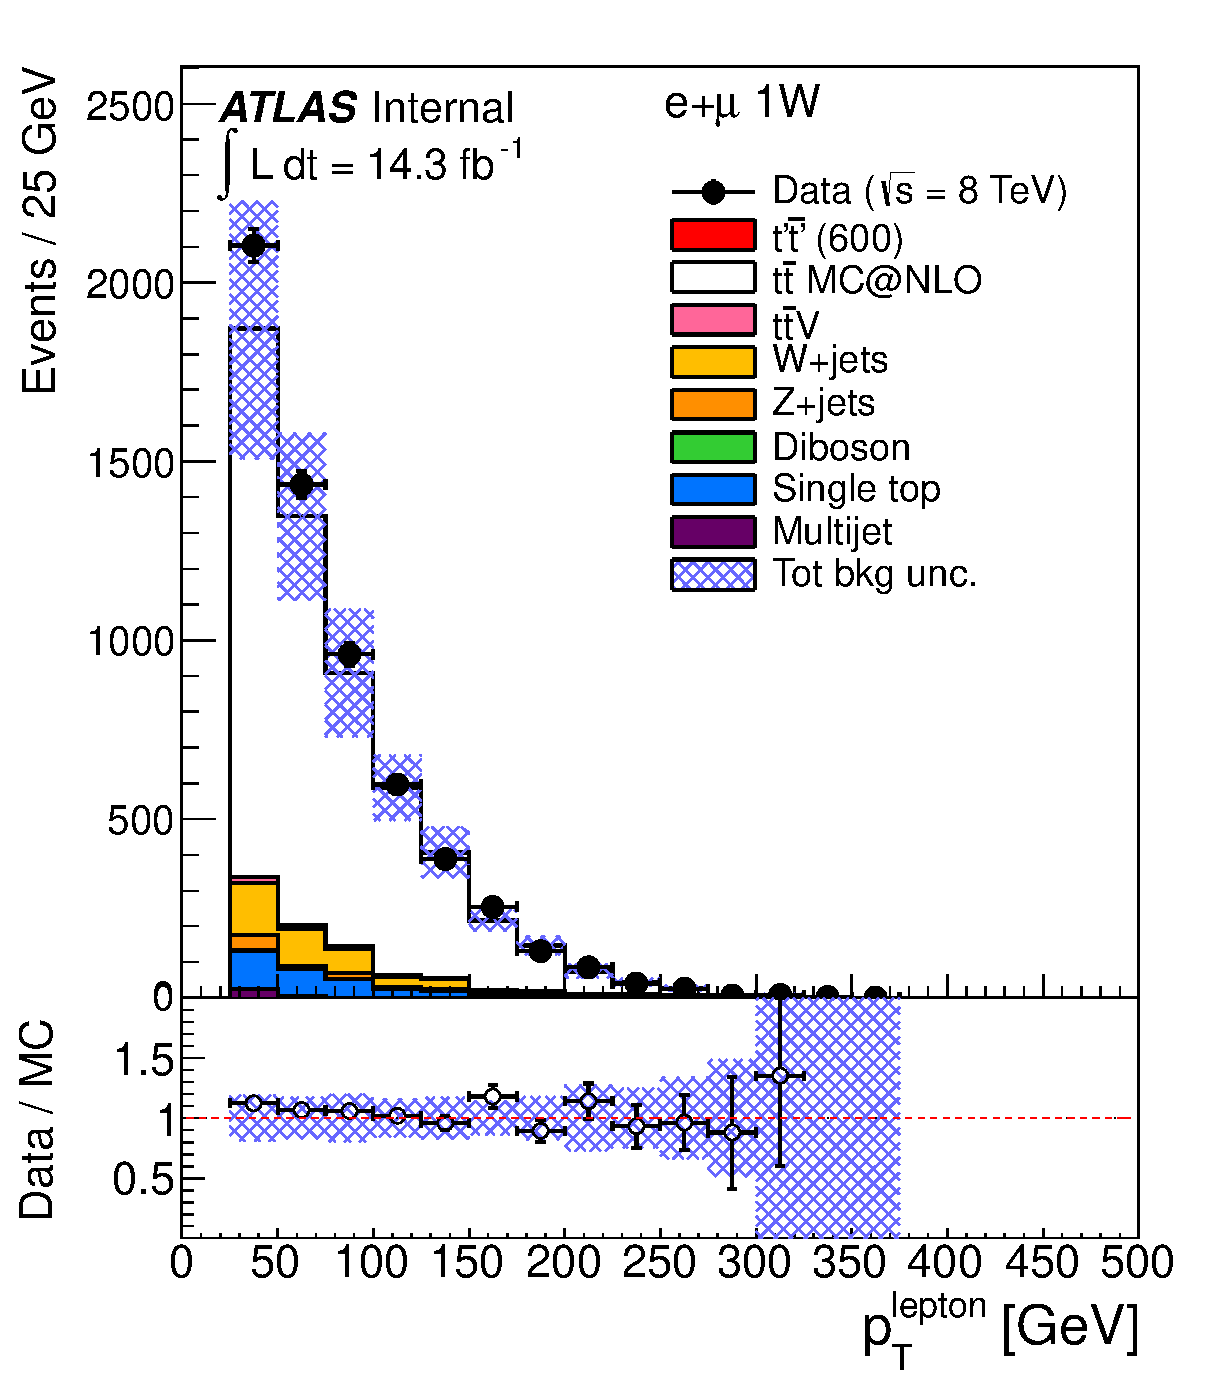
\includegraphics[width=0.3\textwidth]{appendices/figures/sdrs/LepPt_ELEMUONCR0_1W_NOMINAL.eps}}
	\subfigure[]{
          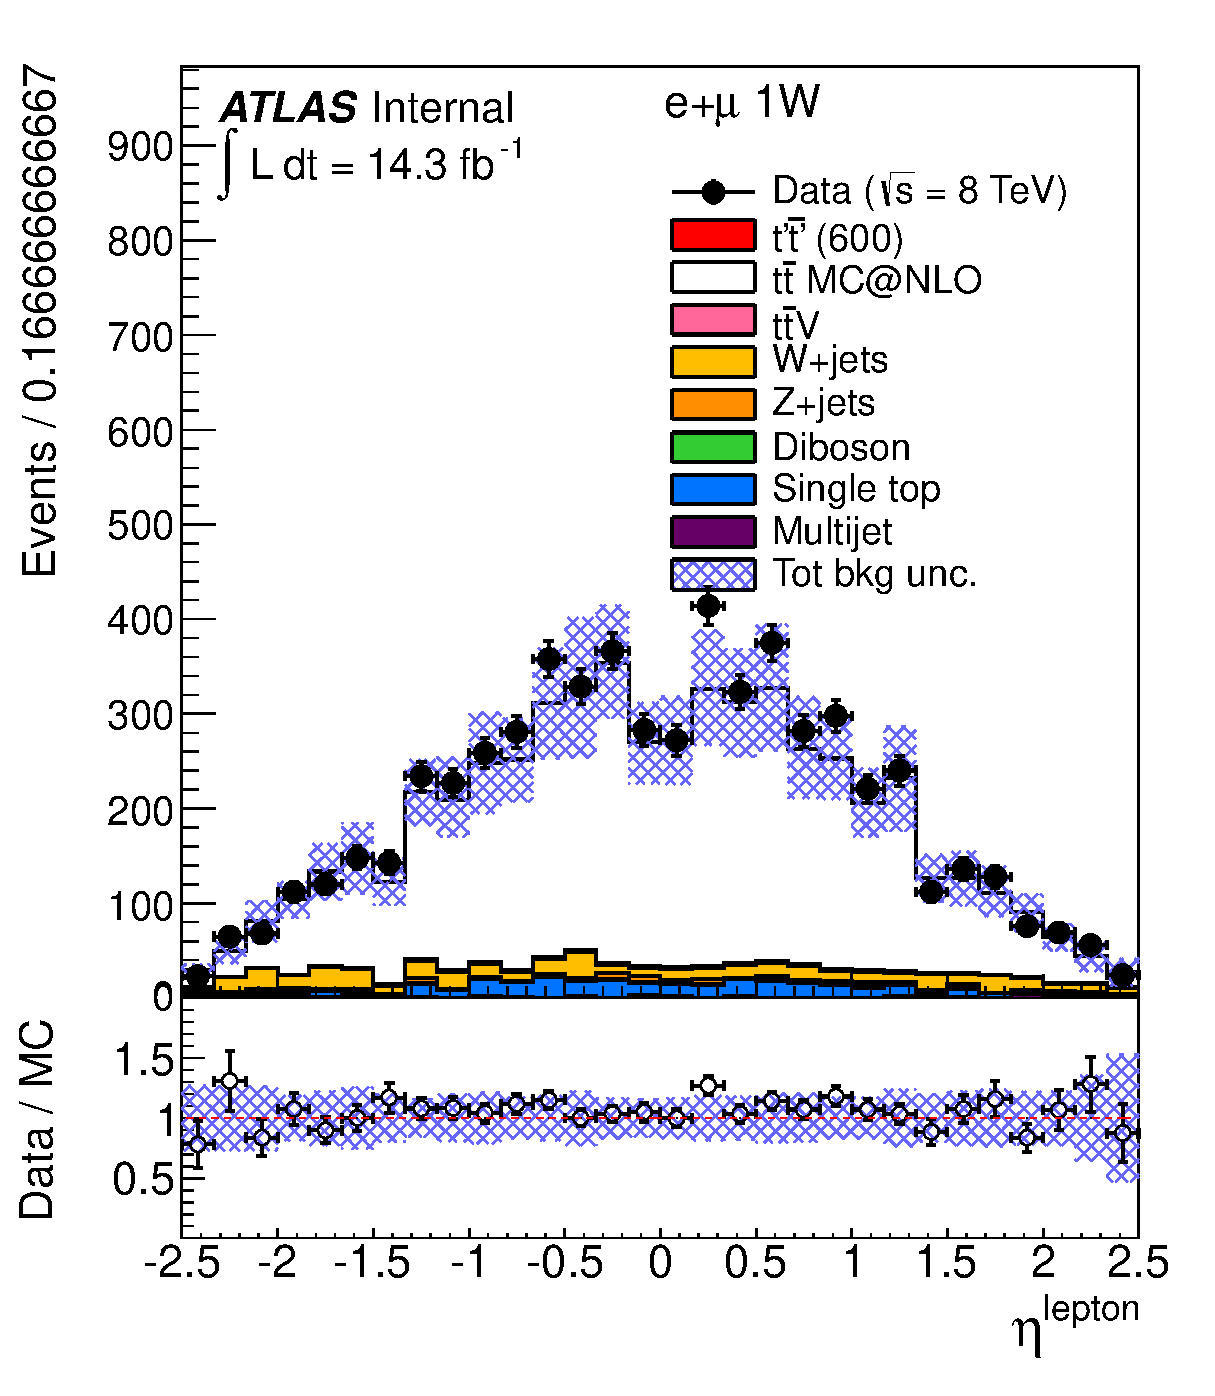
\includegraphics[width=0.3\textwidth]{appendices/figures/sdrs/LepEta_ELEMUONCR0_1W_NOMINAL.eps}}
	\subfigure[]{
          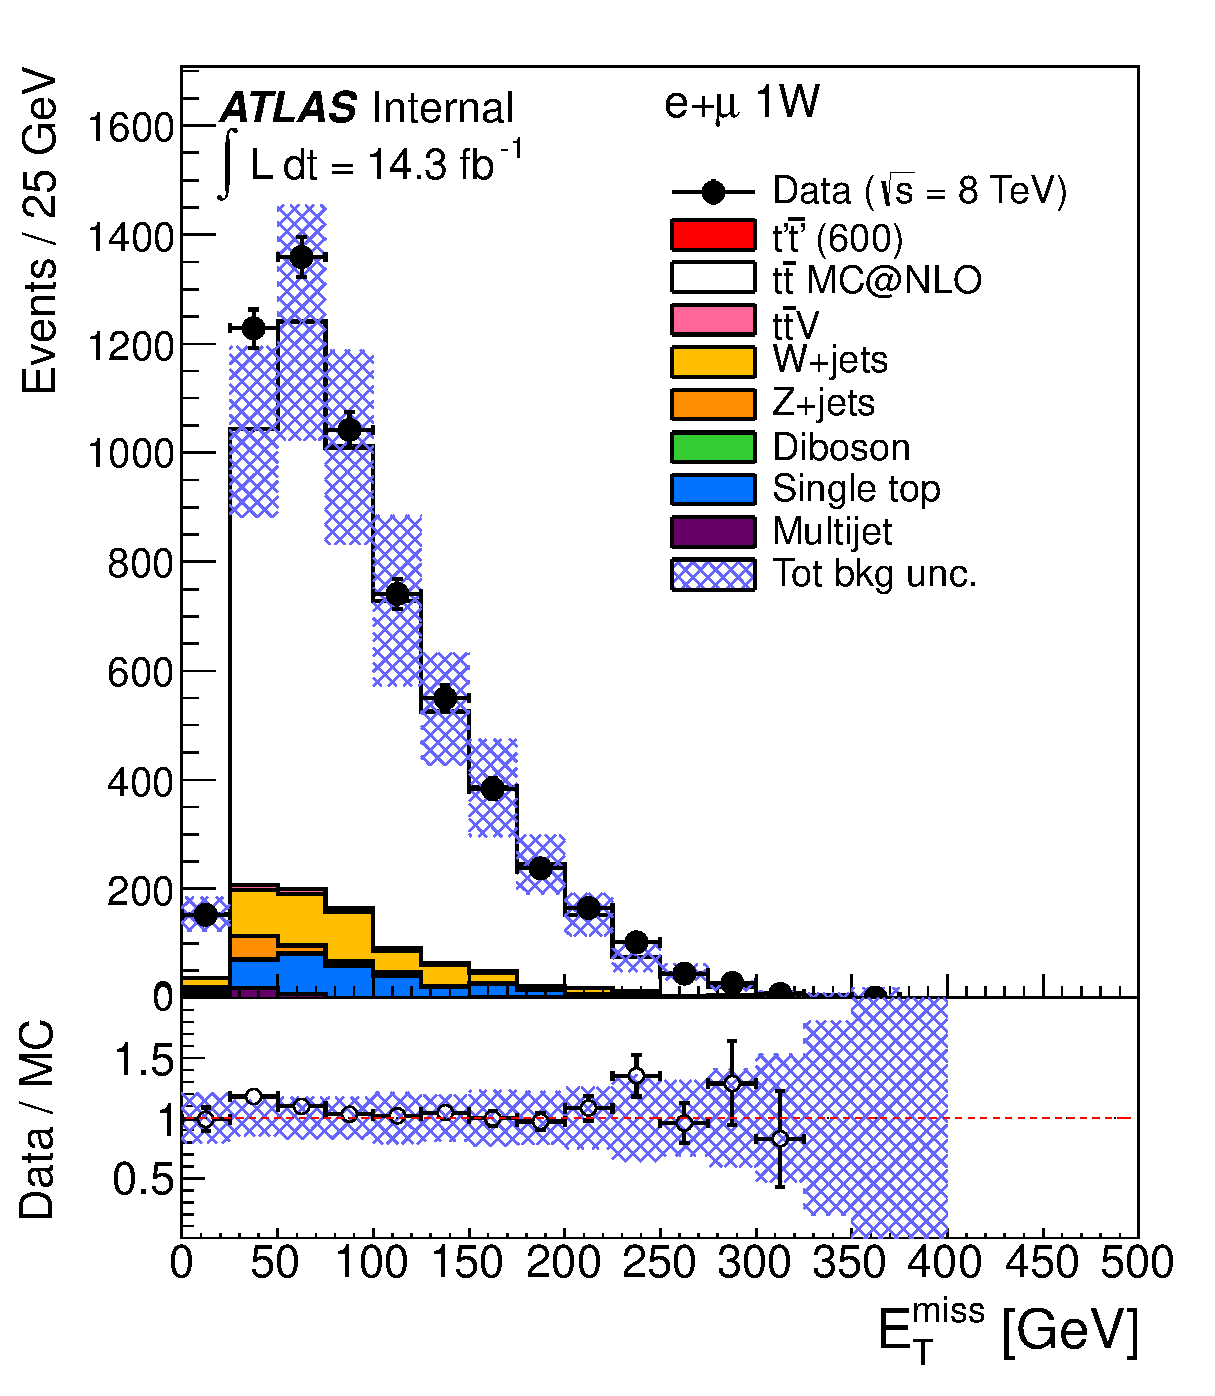
\includegraphics[width=0.3\textwidth]{appendices/figures/sdrs/MET_ELEMUONCR0_1W_NOMINAL.eps}}
	\subfigure[]{
          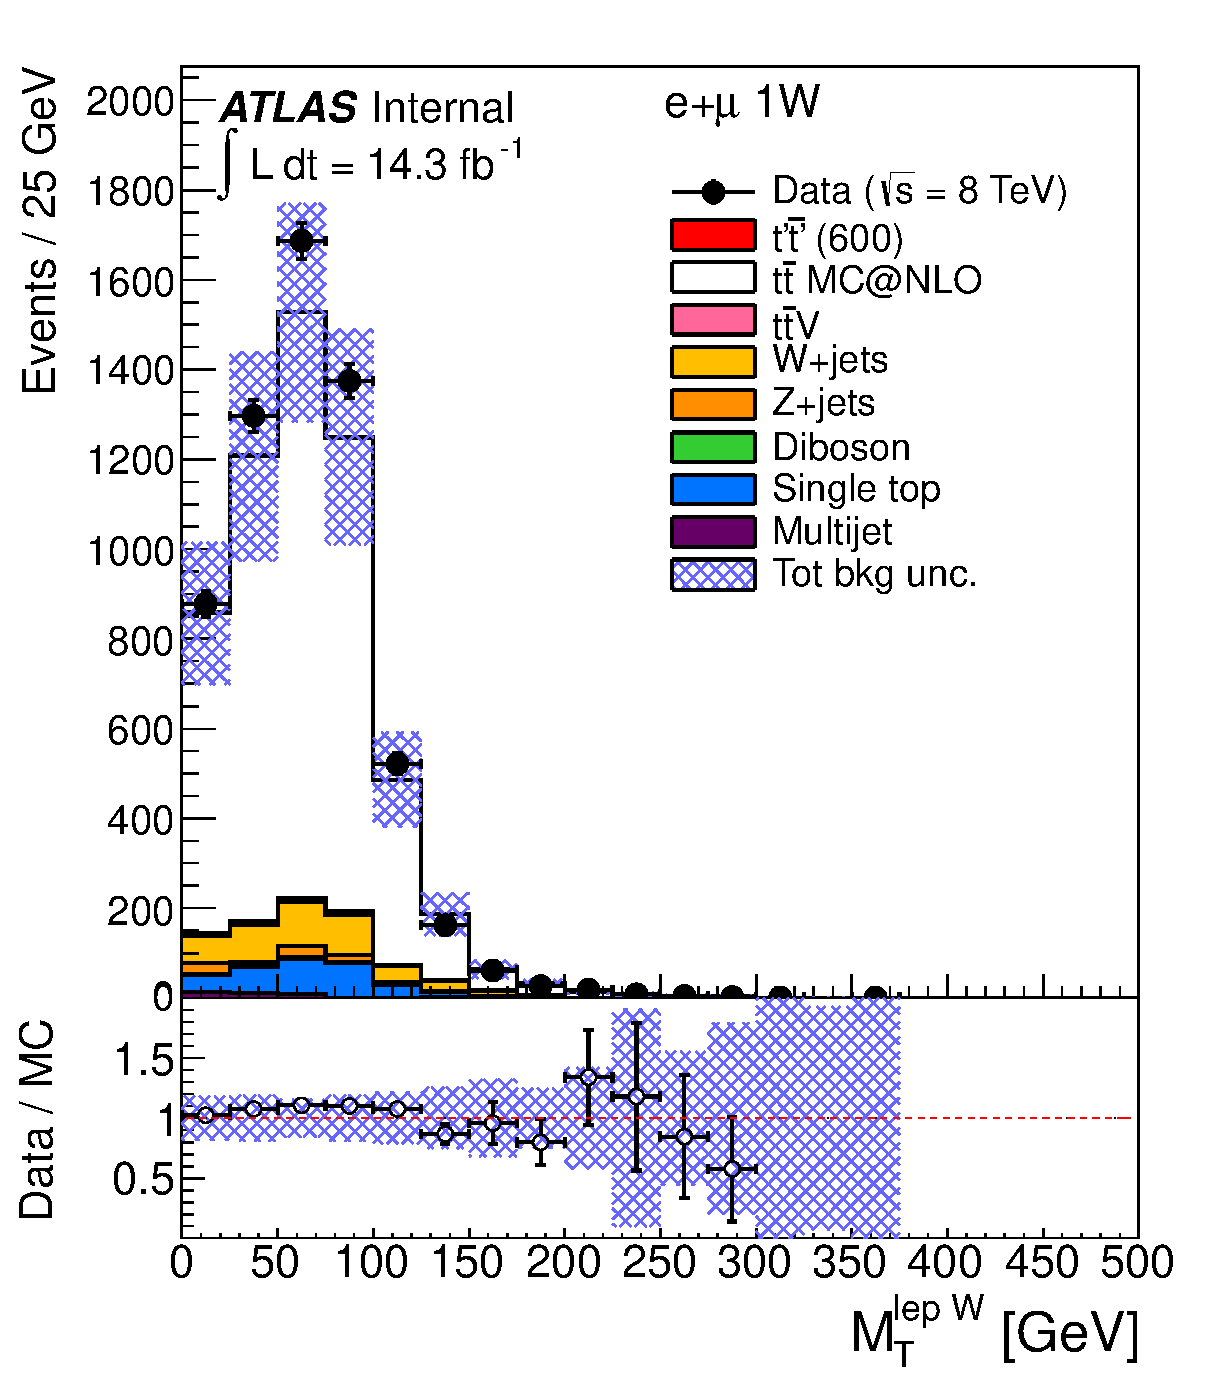
\includegraphics[width=0.3\textwidth]{appendices/figures/sdrs/Wlep_MassT_ELEMUONCR0_1W_NOMINAL.eps}}
	\subfigure[]{
          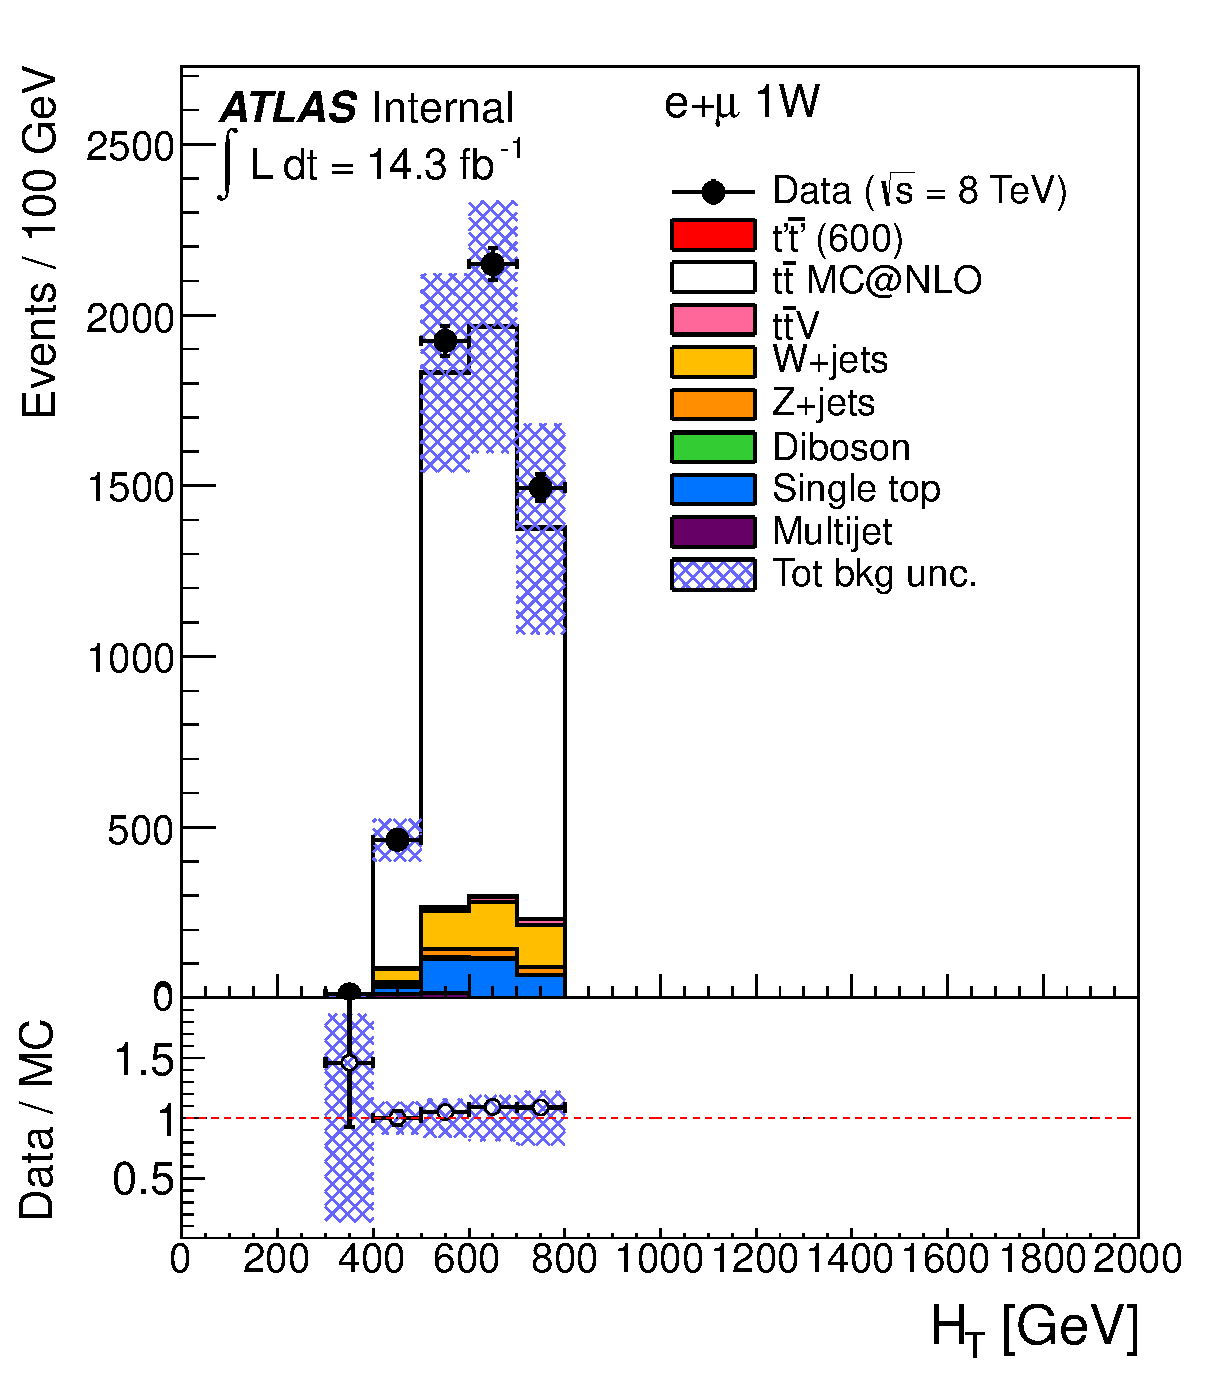
\includegraphics[width=0.3\textwidth]{appendices/figures/sdrs/HTAll_ELEMUONCR0_1W_NOMINAL.eps}}
}\\
\hskip-2cm
\resizebox{1.5\textwidth}{!}{
	\subfigure[]{
          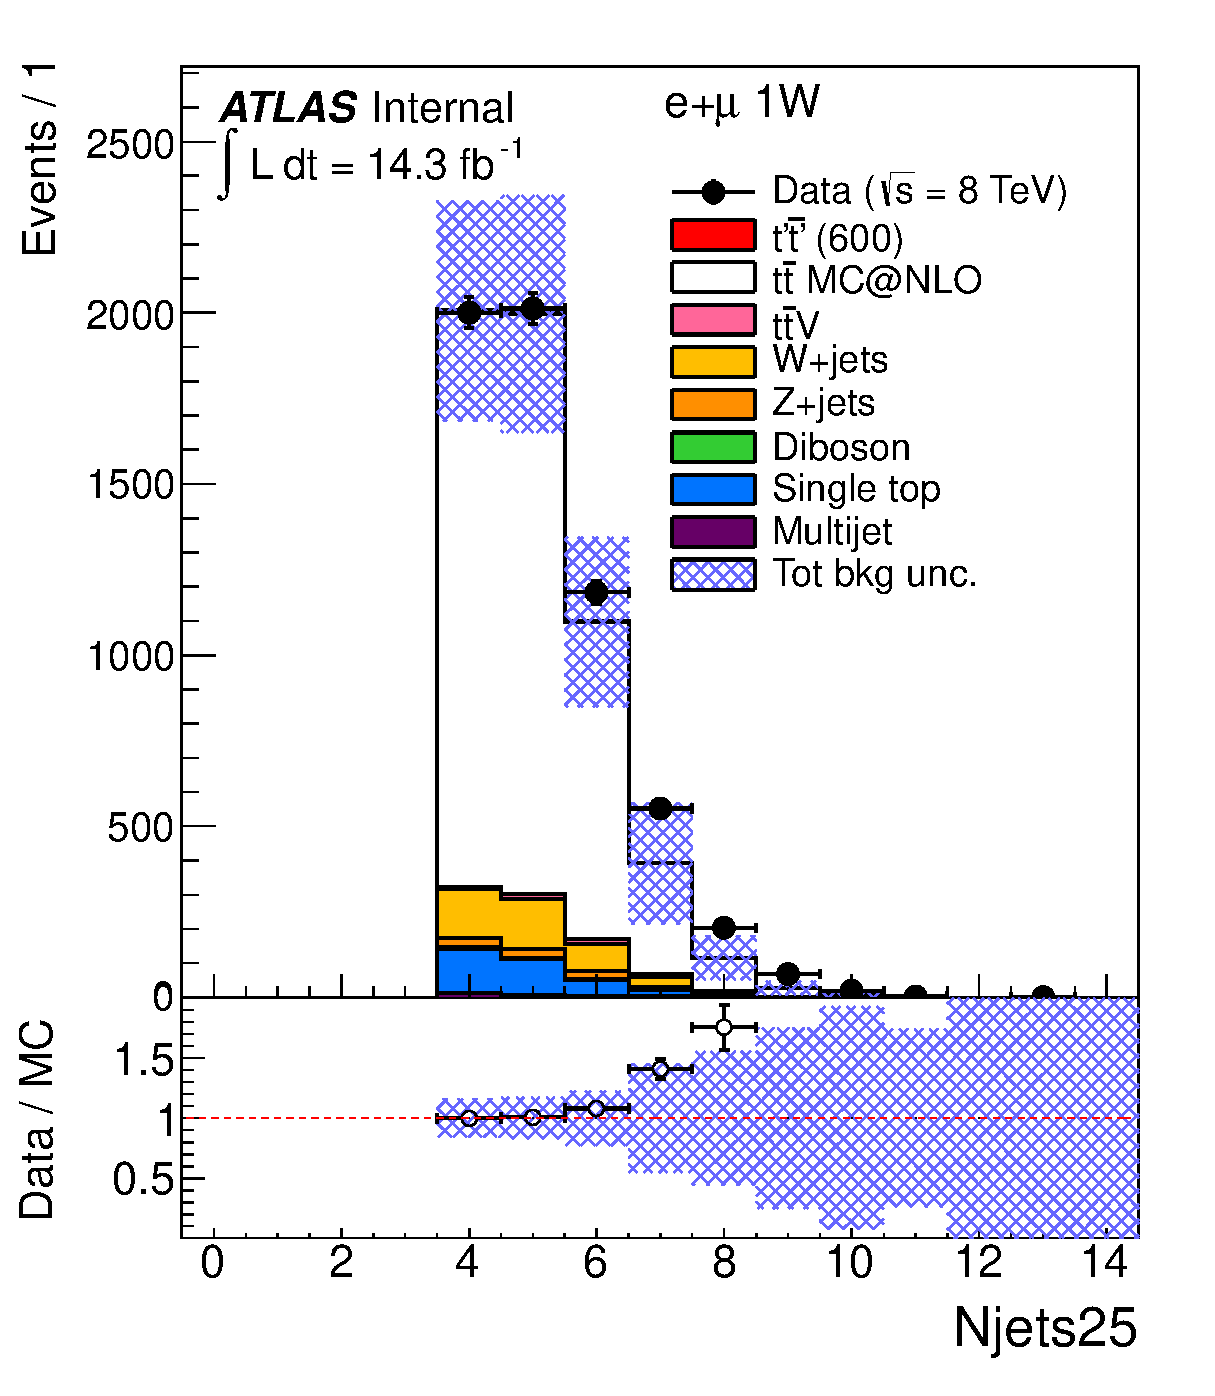
\includegraphics[width=0.3\textwidth]{appendices/figures/sdrs/Njets25_ELEMUONCR0_1W_NOMINAL.eps}}
	\subfigure[]{
          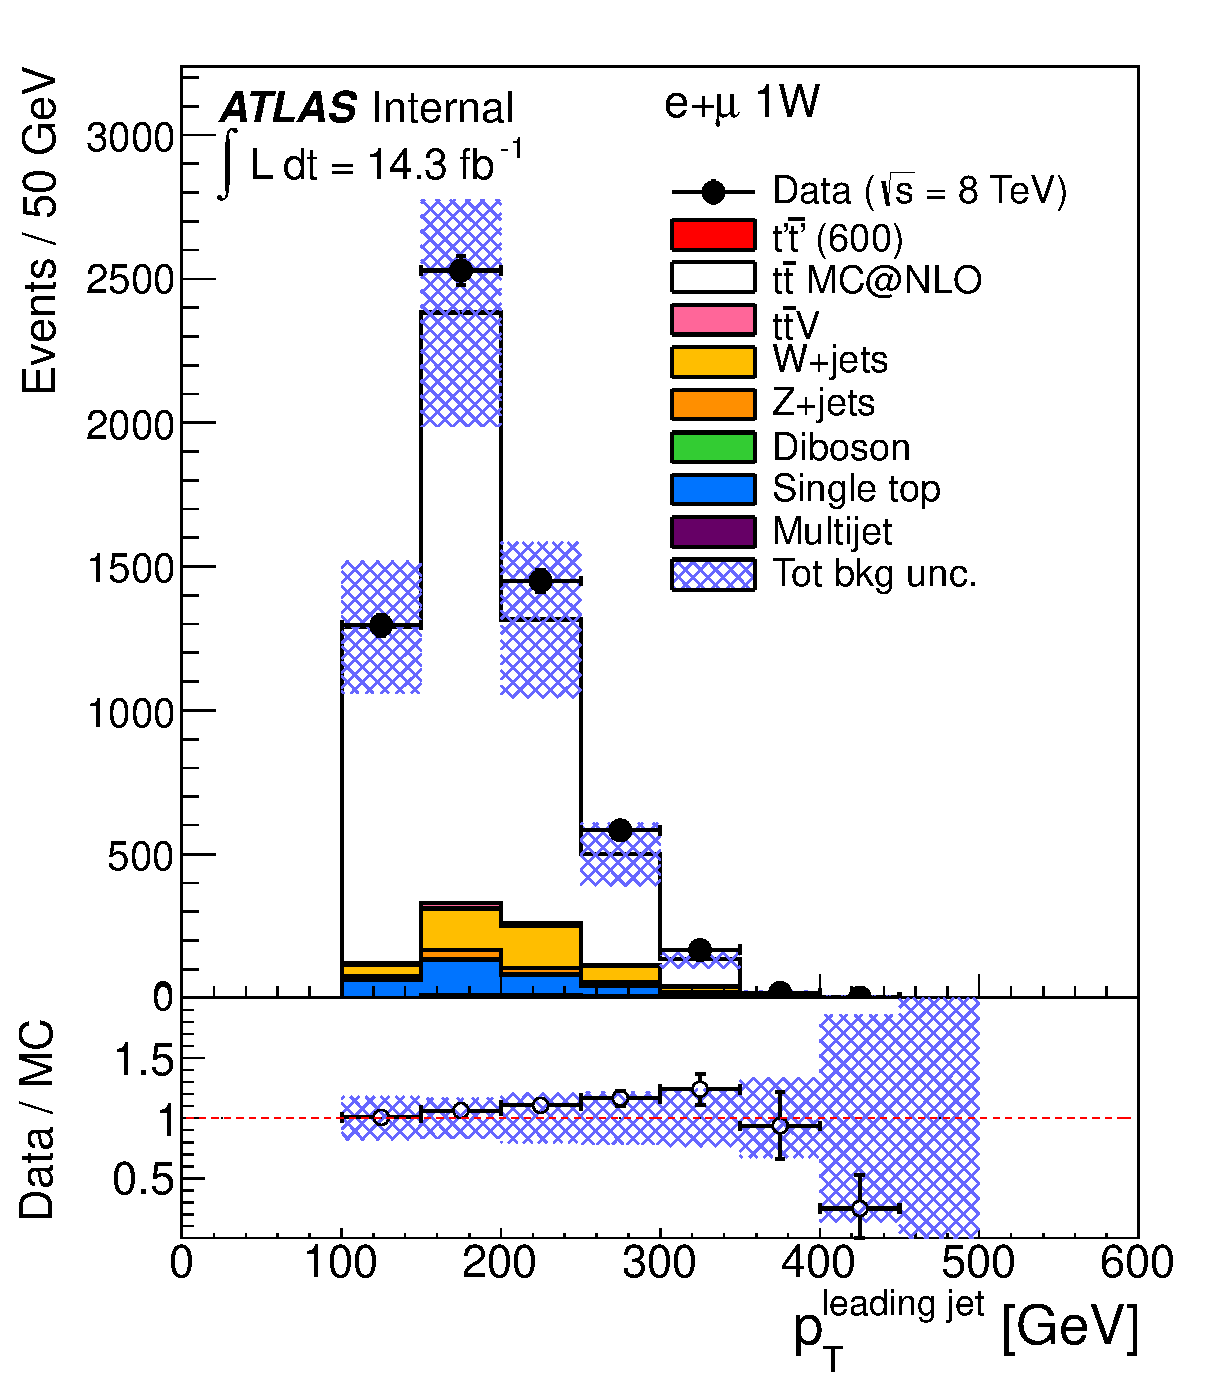
\includegraphics[width=0.3\textwidth]{appendices/figures/sdrs/JetPt1_ELEMUONCR0_1W_NOMINAL.eps}}
	\subfigure[]{
          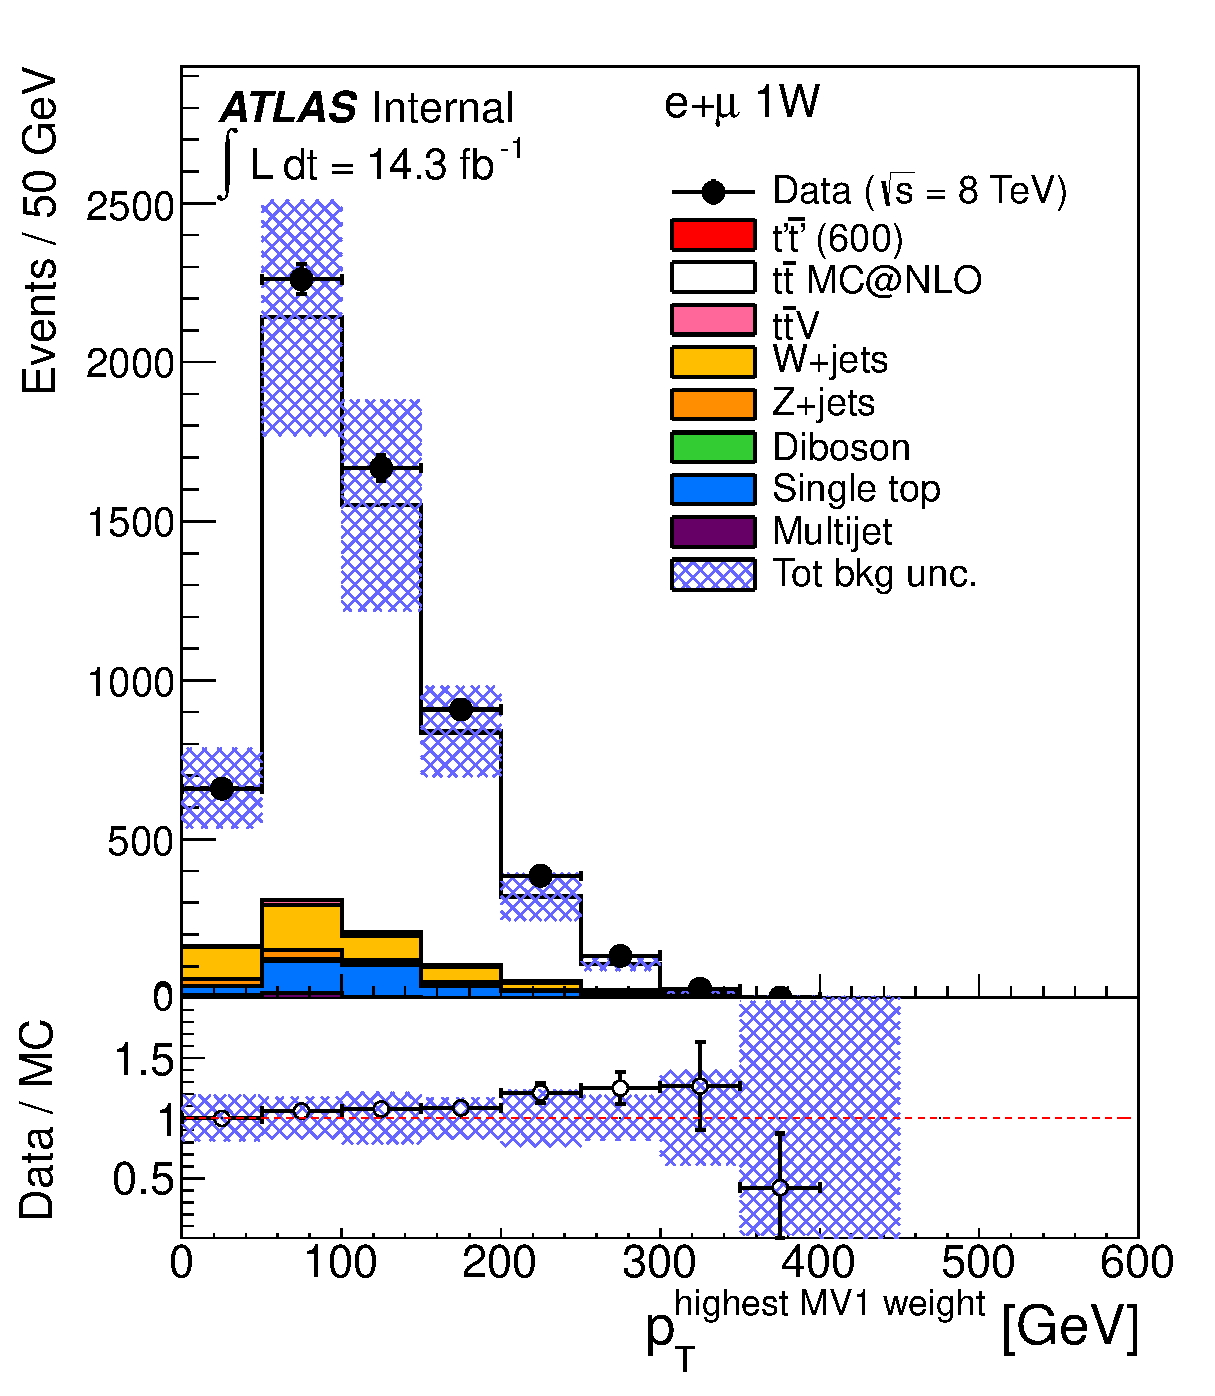
\includegraphics[width=0.3\textwidth]{appendices/figures/sdrs/JetPtB1_ELEMUONCR0_1W_NOMINAL.eps}}
	\subfigure[]{
          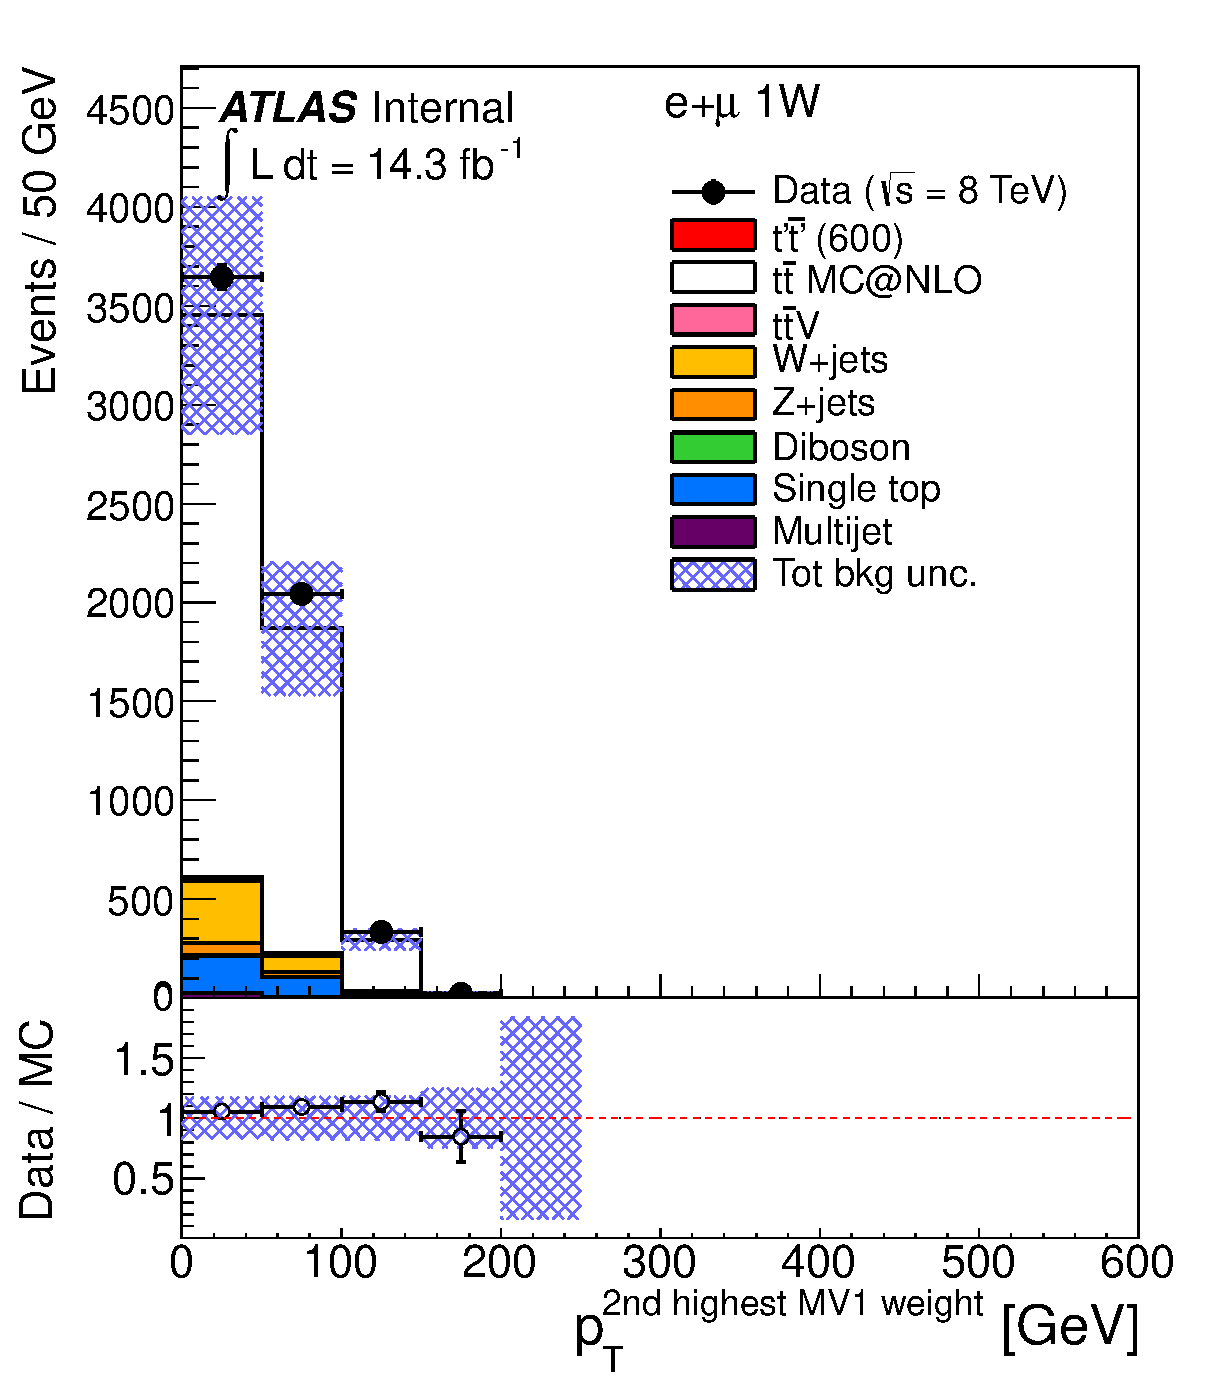
\includegraphics[width=0.3\textwidth]{appendices/figures/sdrs/JetPtB2_ELEMUONCR0_1W_NOMINAL.eps}}
	\subfigure[]{
          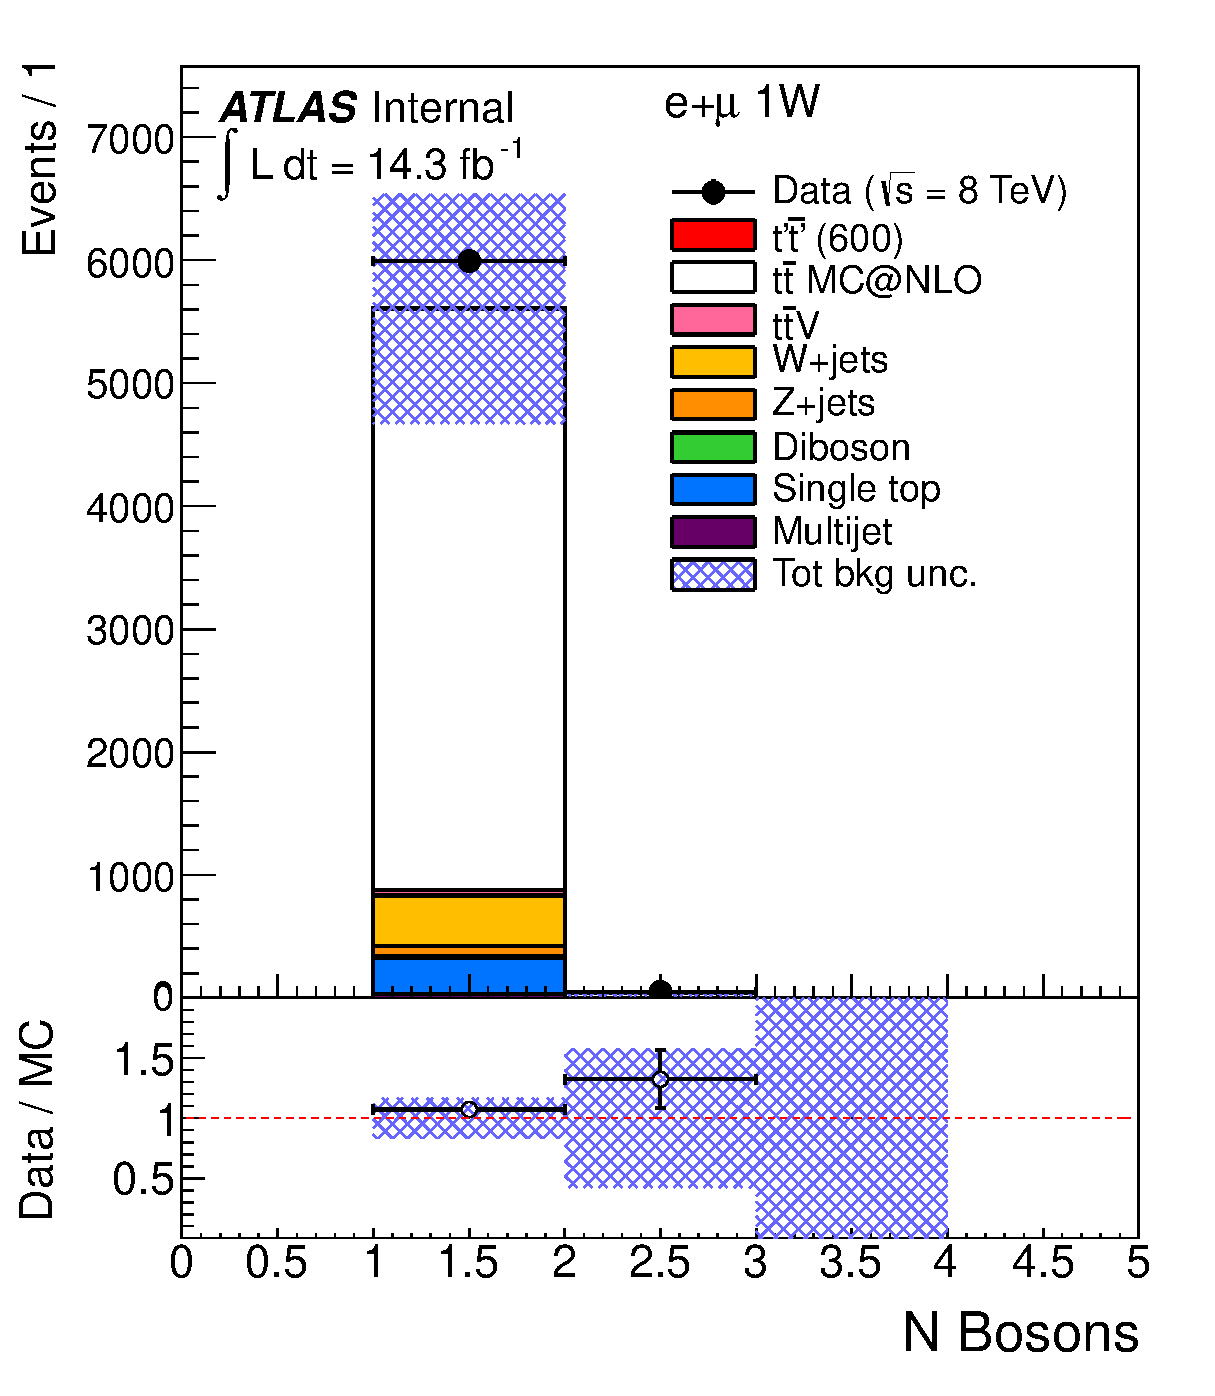
\includegraphics[width=0.3\textwidth]{appendices/figures/sdrs/nWhad_ELEMUONCR0_1W_NOMINAL.eps}}
}\\
\hskip-2cm
\resizebox{1.5\textwidth}{!}{
	\subfigure[]{
          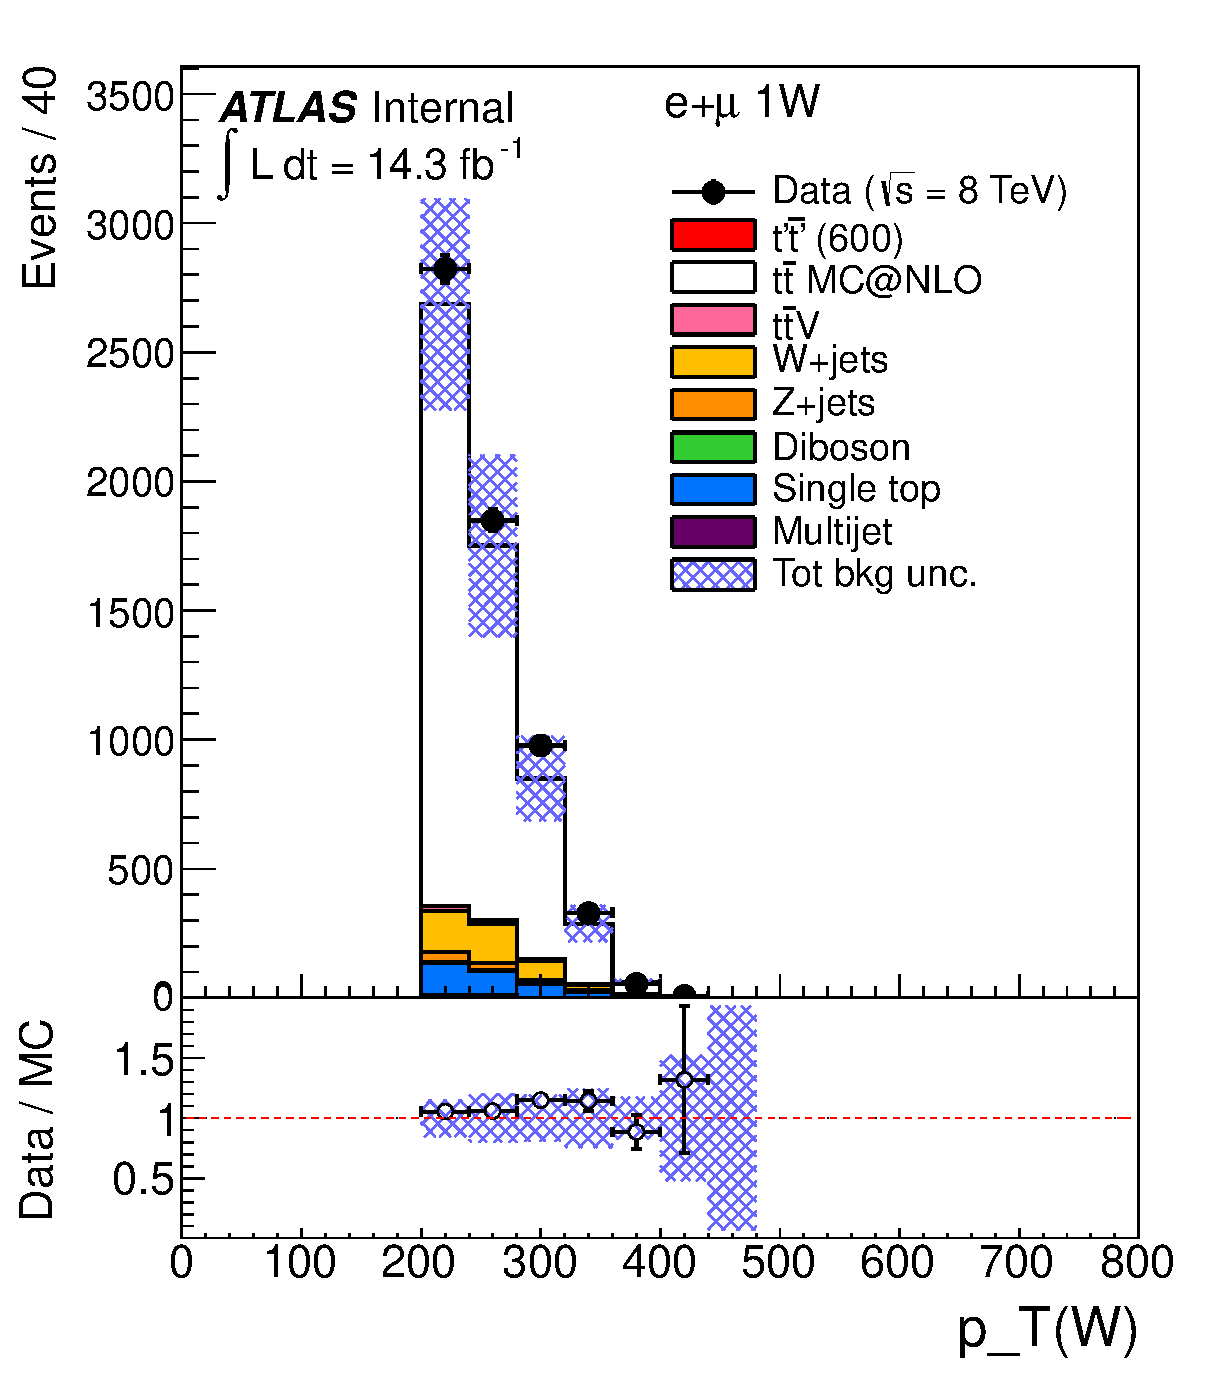
\includegraphics[width=0.3\textwidth]{appendices/figures/sdrs/VLQAna_WbX_W1Pt_ELEMUONCR0_1W_NOMINAL.eps}}
	\subfigure[]{
          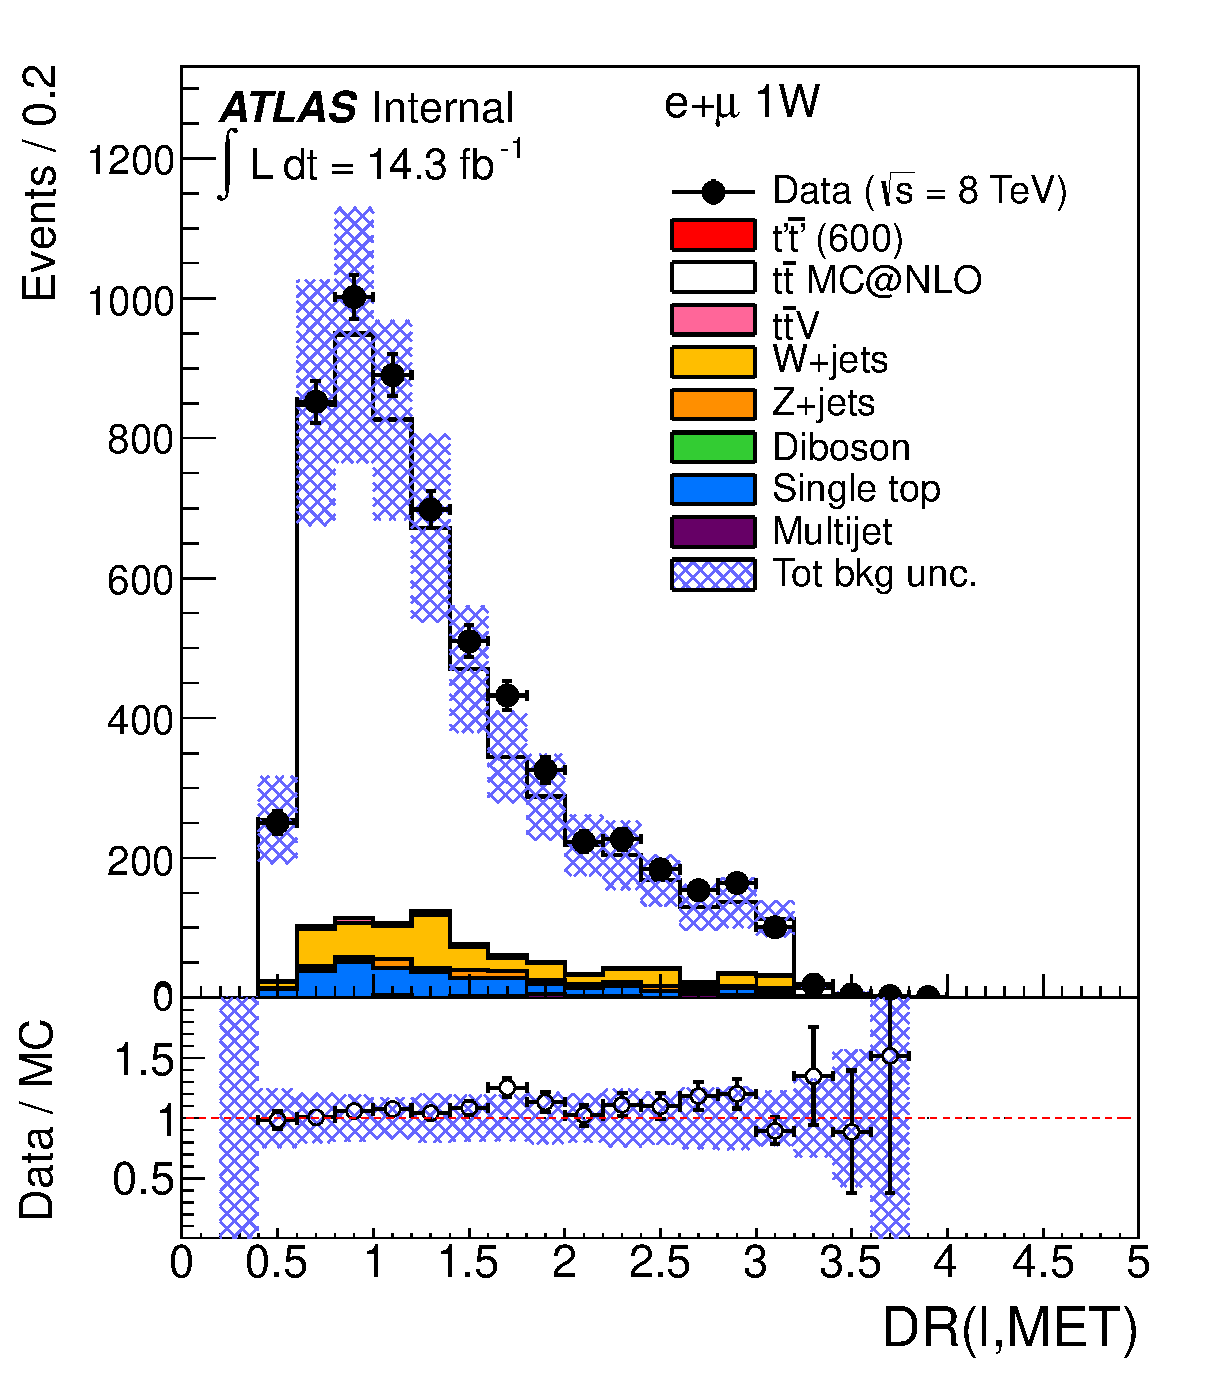
\includegraphics[width=0.3\textwidth]{appendices/figures/sdrs/VLQAna_WbX_DRLepMet_ELEMUONCR0_1W_NOMINAL.eps}}
	\subfigure[]{
          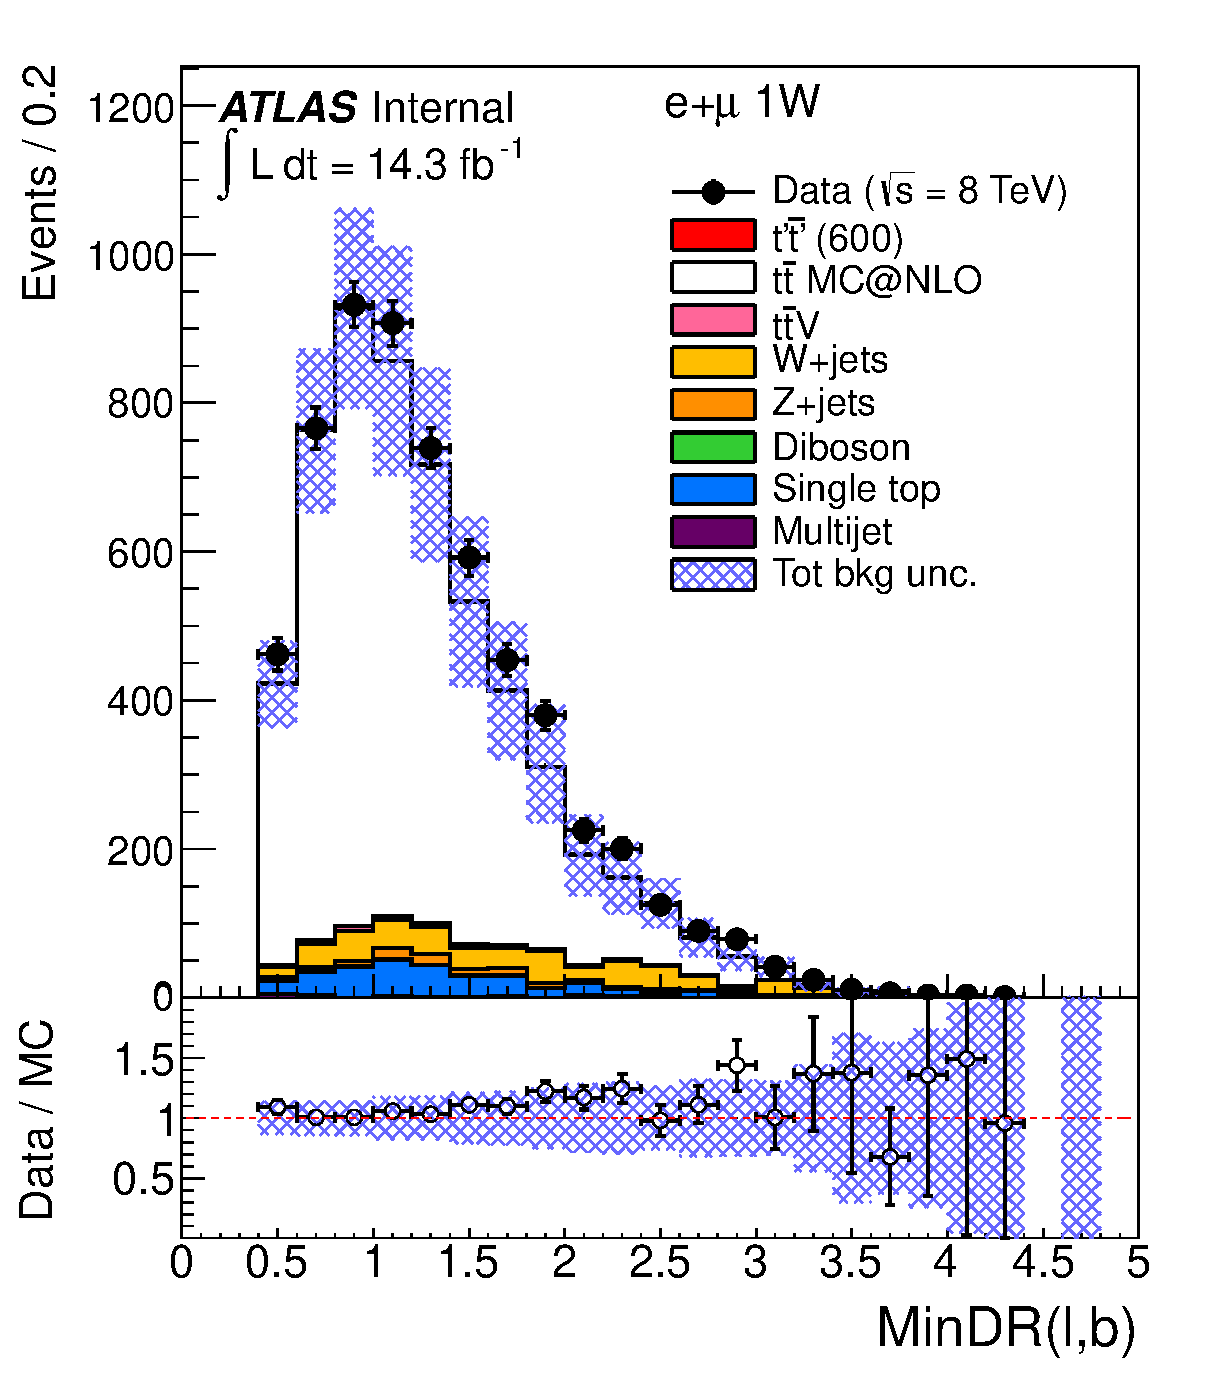
\includegraphics[width=0.3\textwidth]{appendices/figures/sdrs/VLQAna_WbX_MinDRlb_ELEMUONCR0_1W_NOMINAL.eps}}
	\subfigure[]{
          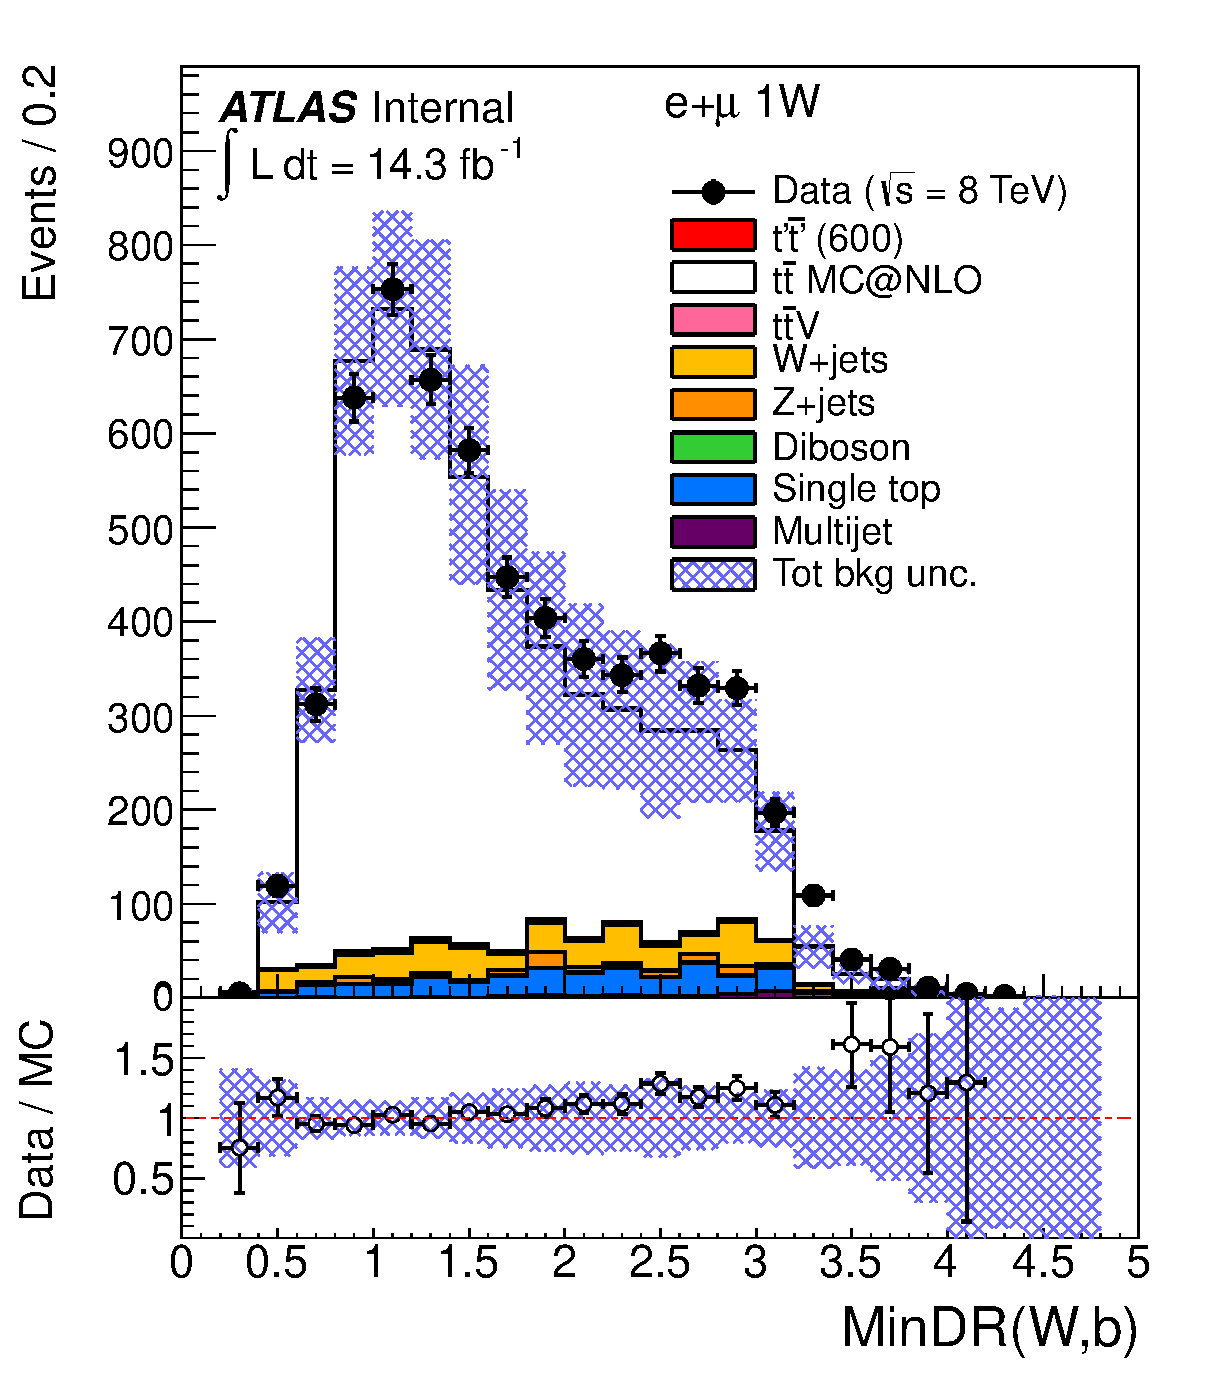
\includegraphics[width=0.3\textwidth]{appendices/figures/sdrs/VLQAna_WbX_MinDRWb_ELEMUONCR0_1W_NOMINAL.eps}}
	\subfigure[]{
          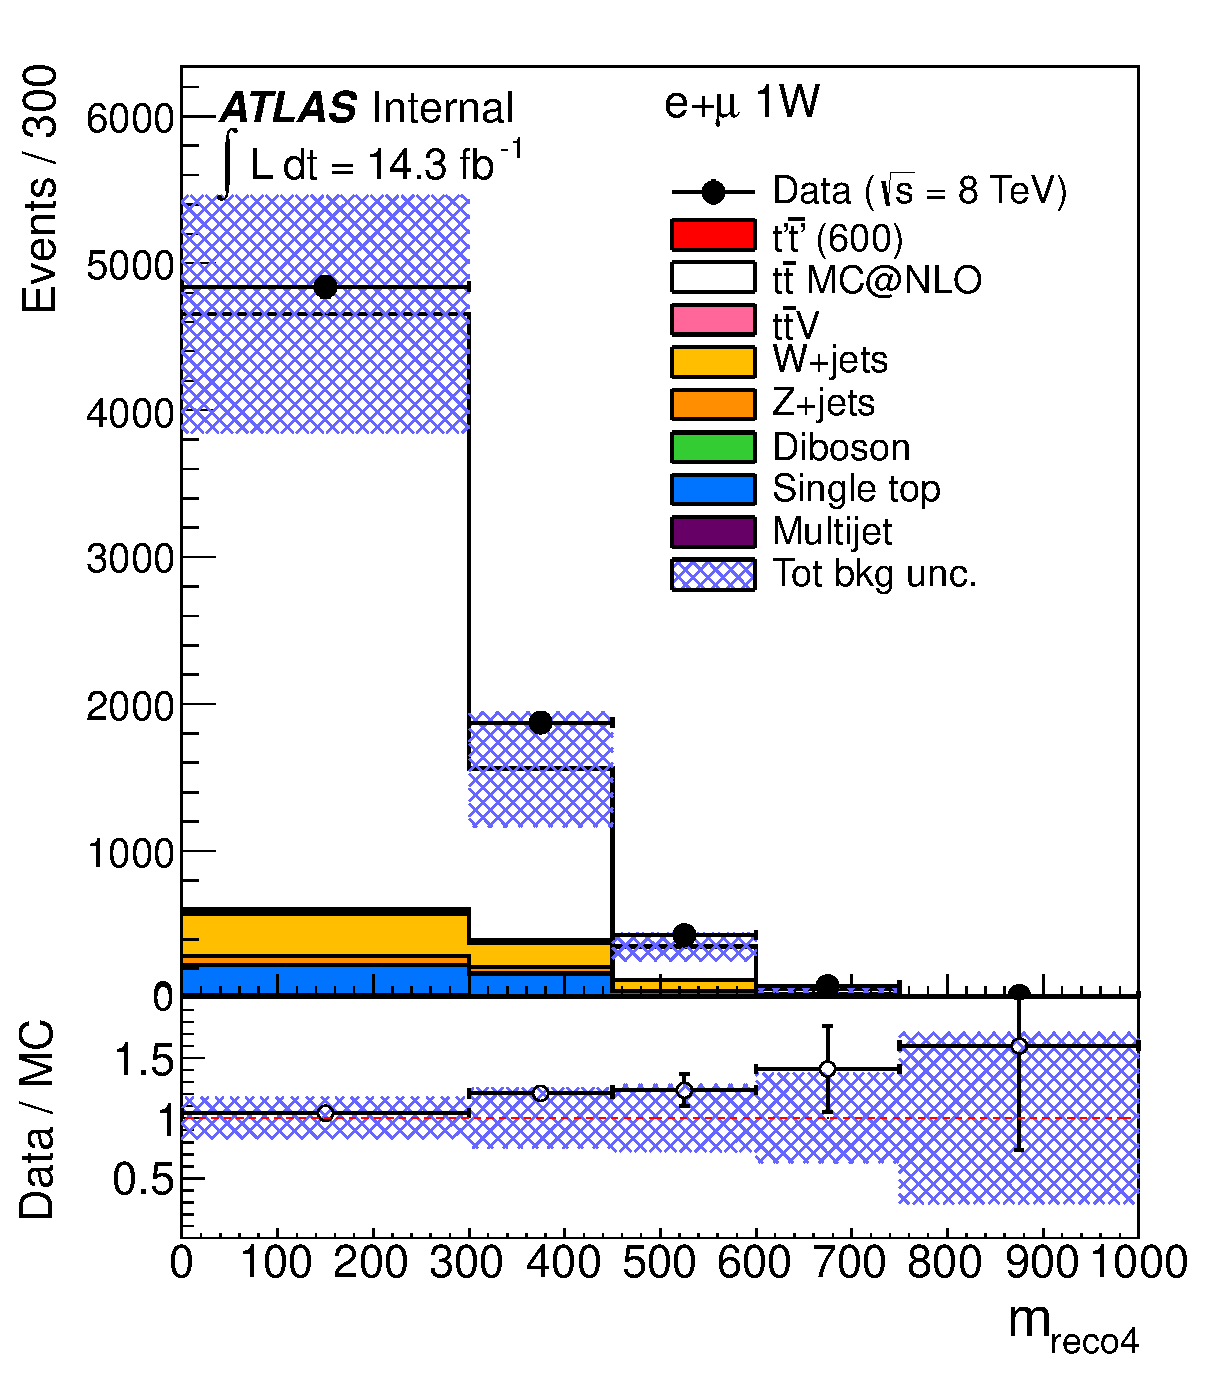
\includegraphics[width=0.3\textwidth]{appendices/figures/sdrs/VLQAna_WbX_1W_MWb_4_ELEMUONCR0_1W_NOMINAL.eps}}
}
	\caption{Comparison between data and prediction in combined $e$+jets and $\mu$+jets combined channel in SDR0
          for a number of kinematic variables: 
          %%%row 1
          (a)  lepton $\pt$, (b) lepton $\eta$, (c) missing transverse energy, 
          (d)  $W$ transverse mass, (e) $\HT$ variable, 
          %%%row 2
          (f) number of jets with $\pt>25\gev$, (g) leading jet $\pt$, 
          (h) $\pt$ for leading \bjet, (i) $\pt$ for second-leading \bjet,
          (j) number of $W_{\rm had}$  candidates, 
          %%%row 3
          (k) $\pt$ of selected $W_{\rm had}$  candidate, 
          (l) $\Delta R(\ell,\nu)$, (m) $\min(\Delta R(\ell, b_{1,2}))$, 
          (n) $\min(\Delta R(W_{\rm had}, b_{1,2}))$ and (o) $m_{\rm reco}$.
          The shaded area represents the total background uncertainty.\label{fig:ELEMUONCR0}}
\end{center}\end{figure}
\end{landscape}
